%% Report layout adapted from the Computer Science report template
%% (Dr Todd R. Jones, University of Reading, based on a template by Dr Varun Ojha),
%% as required by the course. The template's CS_report.sty settings are included
%% below so that the whole report lives in this file.
\documentclass[a4paper,11pt,oneside]{book}

%% ----- Template settings (CS_report.sty) -----
\usepackage[margin=1.2in]{geometry}

% Sans-serif font
\usepackage[T1]{fontenc}
\usepackage{lmodern}
\renewcommand*\familydefault{\sfdefault}
\usepackage{slantsc}
\usepackage{relsize}
\usefont{T1}{lmss}{m}{n}\selectfont
\DeclareFontShape{T1}{lmss}{m}{sc}{<->ssub*lmss/m/n}{}

% Math
\usepackage{sansmath}
\sansmath
\usepackage[cmex10]{amsmath}
\usepackage{amssymb}
\usepackage{amsthm}

% Code listings
\usepackage[utf8]{inputenc}
\usepackage{listings}
\usepackage{xcolor}
\definecolor{codegreen}{rgb}{0,0.6,0.1}
\definecolor{codegray}{rgb}{0.5,0.5,0.5}
\definecolor{codeblue}{rgb}{0.10,0.00,1.00}
\definecolor{codepurple}{rgb}{0.58,0,0.82}
\definecolor{backcolour}{rgb}{1.0,1.0,1.0}
\lstdefinestyle{mystyle}{
    backgroundcolor=\color{backcolour},
    commentstyle=\color{codegreen},
    keywordstyle=\color{codeblue},
    numberstyle=\tiny\color{codegray},
    stringstyle=\color{codepurple},
    basicstyle=\ttfamily\footnotesize,
    breakatwhitespace=false,
    breaklines=true,
    captionpos=b,
    keepspaces=true,
    numbers=left,
    numbersep=5pt,
    showspaces=false,
    showstringspaces=false,
    showtabs=false,
    tabsize=2,
    frame=none
}
\lstset{style=mystyle}

% Figures and tables
\usepackage{graphicx}
\usepackage{caption}
\usepackage{multirow}
\usepackage{rotating}
\usepackage{makecell}
\usepackage{booktabs}

% List of abbreviations
\usepackage{enumitem}
\newlist{abbrv}{itemize}{1}
\setlist[abbrv,1]{label=,labelwidth=1in,align=parleft,itemsep=0.1\baselineskip,leftmargin=!}

% Links and references
\usepackage[hidelinks]{hyperref}
\usepackage[nameinlink]{cleveref}
\definecolor{DarkBlue}{rgb}{0.00,0.00,0.50}
\hypersetup{colorlinks=true,
            linkcolor=blue,
            filecolor=magenta,
            urlcolor=cyan,
            citecolor=DarkBlue,
            pdftitle={Tsunami Monitoring System -- Workshop 1},
            }

% Bibliography: the template's numbered style (natbib numbers)
\usepackage[numbers]{natbib}
\usepackage[nottoc]{tocbibind}
\renewcommand{\bibname}{References}

% Appendices
\usepackage[toc]{appendix}

%% ----- Additions for this report -----
\usepackage{tabularx}
\usepackage{float}
\renewcommand{\arraystretch}{1.25}
% Long file names and code words: allow looser lines and breaks in paths at _ and .
\setlength{\emergencystretch}{3em}
\expandafter\def\expandafter\UrlBreaks\expandafter{\UrlBreaks\do\_\do\.}

% Red reminder. Search for "TODO" before submitting.
\providecommand{\todo}[1]{\textcolor{red}{[TODO: #1]}}

\begin{document}

    \captionsetup[figure]{margin=1.5cm,font=small,name={Figure},labelsep=colon}
    \captionsetup[table]{margin=1.5cm,font=small,name={Table},labelsep=colon}

    \frontmatter

    % -------------------------------------------------------------------
    % Title page
    % -------------------------------------------------------------------
    \begin{titlepage}
        \begin{center}
            
\includegraphics[width=3cm]{figures/ud.png}\\[0.5cm]
            {\LARGE Universidad Distrital Francisco Jos\'e de Caldas\\[0.5cm]
            School of Engineering -- Computer Engineering Program}\\[2cm]

            \linespread{1.2}\huge {
                Tsunami Monitoring System\\[0.3cm]
                \Large Workshop No.\ 1: Hazard Definition, Source Validation, and Data Contract
            }
            \linespread{1}~\\[2cm]

            {\Large Team 8}\\[0.5cm]
            {\large
            \begin{tabular}{ll}
                Lina Moreno & 20231020133 \\
                Jaider \'Avila & 20231020200 \\
                Gabriela Mart\'inez & 20231020205 \\
            \end{tabular}}\\[1cm]

            {\large \emph{Professor:} Eng.\ Carlos Andr\'es Sierra, M.Sc.}\\[1cm]

            \large A report submitted for Workshop No.\ 1 of the course\\
            \textit{Data Analysis Programming}, Semester 2026-II\\[0.3cm]
            \small
            Repository: \url{https://github.com/g8martinezsilva/tsunami-monitoring}\\[0.2cm]
            Source profiling notebook:\\
            {\scriptsize\url{https://github.com/g8martinezsilva/tsunami-monitoring/blob/main/notebooks/01_source_profiling.ipynb}}\\[0.2cm]
            Canonical mapping table:\\
            {\scriptsize\url{https://github.com/g8martinezsilva/tsunami-monitoring/blob/main/workshop_1/mapping.md}}
            \vfill

            \today
        \end{center}
    \end{titlepage}

    % -------------------------------------------------------------------
    % Declaration
    % -------------------------------------------------------------------
    \newpage
    \thispagestyle{empty}
    \chapter*{\Large Declaration}
    We, Lina Moreno, Jaider \'Avila and Gabriela Mart\'inez, of the Computer Engineering Program, Universidad Distrital Francisco Jos\'e de Caldas, confirm that this is our own work and that figures, tables, equations, code snippets and illustrations in this report are original and have not been taken from any other person's work, except where the works of others have been explicitly acknowledged, quoted, and referenced. Data from external sources are cited with their licenses.
    ~\\[1cm]
    \begin{flushright}
    Lina Moreno\\
    Jaider \'Avila\\
    Gabriela Mart\'inez

    \today
    \end{flushright}

    % -------------------------------------------------------------------
    % Abstract
    % -------------------------------------------------------------------
    \chapter*{Abstract}
    \addcontentsline{toc}{chapter}{Abstract}
    This report defines the Workshop~1 foundation of a monitoring system for tsunami-relevant earthquakes in the Pacific basin.
The scope combines three Marine Regions maritime regions with a 100~km margin, the period 2010--2025, and earthquakes of magnitude 6 or more for historical analysis.
Four free sources were validated with real samples: the NOAA/NCEI HazEL historical tsunami database (221 events), the USGS FDSN earthquake catalog (343 events in the 2010--2011 sample), the USGS real-time feed (four snapshots) and the NTWC/PTWC tsunami.gov bulletins.
Profiling showed four timestamp formats, magnitude types that differ across sources, frequent and late revisions of earthquake records (up to 29 days after the event), an origin date one day off in a PTWC bulletin, and a bulletin that expires before it was sent.
The sources are mapped to a canonical event model with domain tables, and an ingestion contract defines partitioning, watermarks and duplicate keys per source.
Finally, a Tsunami Relevance Level indicator (LOW, MODERATE, HIGH) is proposed as a monitoring aid, not as a tsunami prediction.

    % -------------------------------------------------------------------
    % Contents, list of figures, list of tables, abbreviations
    % -------------------------------------------------------------------
    \tableofcontents
    \listoffigures
    \listoftables

    \chapter*{List of Abbreviations}
    \chaptermark{List of Abbreviations}
    \begin{abbrv}
        \item[CAP]      Common Alerting Protocol
        \item[CRS]      Coordinate Reference System
        \item[FDSN]     International Federation of Digital Seismograph Networks
        \item[GOAS]     Global Oceans and Seas (Marine Regions dataset)
        \item[HazEL]    NCEI Hazard Event Database (Global Historical Tsunami Database interface)
        \item[NCEI]     NOAA National Centers for Environmental Information
        \item[NOAA]     National Oceanic and Atmospheric Administration
        \item[NTWC]     National Tsunami Warning Center (Palmer, Alaska)
        \item[NWS]      National Weather Service
        \item[PTWC]     Pacific Tsunami Warning Center (Honolulu, Hawaii)
        \item[TRL]      Tsunami Relevance Level (indicator proposed in this report)
        \item[USGS]     United States Geological Survey
        \item[UTC]      Coordinated Universal Time
        \item[VLIZ]     Flanders Marine Institute
        \item[WFS]      Web Feature Service
        \item[WGS84]    World Geodetic System 1984
    \end{abbrv}

    % -------------------------------------------------------------------
    % Main chapters
    % -------------------------------------------------------------------
    \mainmatter

\chapter{Introduction}
\label{ch:introduction}

\section{Project Overview}
\textbf{Title.} Tsunami Monitoring System: Pacific earthquakes in the context of historical tsunamis and official bulletins.

\textbf{Motivation.} Large Pacific earthquakes are reported within minutes, but judging whether one deserves attention requires combining several sources that use different formats, identifiers, times and magnitude types (Sections~\ref{sec:historical}--\ref{sec:profiling}).

\textbf{Goal.} From a data-engineering perspective, the goal is a reproducible pipeline that loads two historical and two incremental sources into one canonical model, with idempotent incremental updates, validation and quarantine (Sections~\ref{sec:mapping} and~\ref{sec:contract}).
From an analytical perspective, the goal is to show what is happening now in the Pacific, compare it with the 2010--2025 record, and summarize each significant earthquake with a tsunami-relevance indicator (Section~\ref{sec:indicator}).

\textbf{Scope.} Pacific maritime regions plus a 100~km margin (Section~\ref{sec:hazard}); historical period 2010--2025; earthquakes with $M \geq 4.5$ for the recent-events view and $M \geq 6$ for statistics and the indicator; official bulletins from NTWC and PTWC.

\textbf{Explicit exclusions.} The system does not predict tsunamis, issue warnings, model wave propagation or inundation, or replace the warning centers.
It does not load run-up observations (Section~\ref{sec:historical}), river and lake tsunamis outside the maritime scope, or Colombian national sources, which would first need demonstrated programmatic access.

\textbf{Constraints.} Only free sources are used, within their rate limits and licenses; tsunami.gov keeps only its latest messages; preliminary magnitudes and locations are revised for weeks (Section~\ref{sec:empirical-updates}); and the whole system must run locally with Docker Compose on the team's laptops.

\textbf{Deliverables.} This report is submitted with the project repository, which contains the other Workshop~1 deliverables:
\begin{itemize}[nosep]
  \item Repository: \url{https://github.com/g8martinezsilva/tsunami-monitoring}
  \item Source profiling notebook:\\ \url{https://github.com/g8martinezsilva/tsunami-monitoring/blob/main/notebooks/01_source_profiling.ipynb}
  \item Canonical mapping table:\\ \url{https://github.com/g8martinezsilva/tsunami-monitoring/blob/main/workshop_1/mapping.md}
\end{itemize}

\section{Hazard Definition}
\label{sec:hazard}

\subsection{Phenomenon and Severity Measure}
\label{sec:severity}
A tsunami is a series of long ocean waves generated by the sudden displacement of a large volume of water.
Most tsunamis are caused by large undersea earthquakes, but landslides, volcanic eruptions and meteorological events can also generate them.
In our HazEL sample, 36 of 221 events (16\%) have a non-earthquake cause (landslide 17, meteorological 9, volcano 6, unknown 2, among others).

Earthquake magnitude is an important measure of the size of a
potential seismic source, but it is not a direct measure of
tsunami severity. Some tsunamis are generated by landslides,
volcanic activity, or meteorological phenomena without an
associated earthquake magnitude.

For seismic events, the system considers magnitude, magnitude
type, depth, and location. Historical tsunami records provide
additional information, including maximum observed water height,
cause, event validity, and documented impacts.

Official tsunami bulletins provide operational assessments through
CAP severity, urgency, and certainty. These categories are not
directly equivalent to earthquake magnitude or measured wave height.

Table~\ref{tab:severity} summarizes these complementary measures.

\begin{table}[H]
\centering
\small
\noindent\begin{tabularx}{\textwidth}{@{}>{\raggedright\arraybackslash}p{3.5cm}>{\raggedright\arraybackslash}p{3.2cm}>{\raggedright\arraybackslash}p{2.6cm}>{\raggedright\arraybackslash}X@{}}
\toprule
Measure & Unit & Source & Meaning \\
\midrule
Earthquake magnitude (\texttt{mag}, \texttt{eqMagnitude}) & Dimensionless; the magnitude type is stored & USGS, HazEL, tsunami.gov & Size of the earthquake that may generate a tsunami \\
Earthquake depth (\texttt{depth}, \texttt{eqDepth}) & km & USGS, HazEL, tsunami.gov & Shallow events are more likely to displace the seafloor \\
Maximum water height (\texttt{maxWaterHeight}) & m & HazEL & Observed tsunami height (historical only) \\
Event validity (\texttt{eventValidity}) & Ordinal scale from $-1$ to $4$ & HazEL & Confidence that the event was a real tsunami, from erroneous or doubtful entry to definite tsunami \\
Official alert (CAP \texttt{severity}, \texttt{certainty}) & Categorical (e.g.\ Minor / Unlikely) & tsunami.gov & Assessment by the warning centers \\
\texttt{tsunami} flag & 0 / 1 & USGS real-time & A tsunami bulletin \emph{may} exist; it does \textbf{not} mean that a tsunami occurred \\
\bottomrule
\end{tabularx}
\caption{Severity-related variables used by the system.}
\label{tab:severity}
\end{table}

\paragraph{Units of the HazEL fields.}
The HazEL API description (Swagger) defines \texttt{eqDepth} only as an integer and does not state units, but the HazEL search forms do~\cite{hazelforms}: the tsunami search lists ``Maximum Water Height (m)'', and the earthquake search lists ``Focal Depth (km)''.
The tsunami \texttt{eqDepth} is the focal depth of the linked NCEI earthquake record: for the 2011 Tohoku tsunami (event 5413), the linked earthquake 9799 (\texttt{earthquakeEventId}) has \texttt{eqDepth} = 29, the same value as the tsunami record.
Therefore \texttt{eqDepth} is in kilometers and \texttt{maxWaterHeight} in meters.
The data agree: in 25 of the 28 NOAA--USGS pairs of the sample (Section 7 of \path{notebooks/01_source_profiling.ipynb}) the HazEL depth is within 2~km of the USGS depth.
Being an integer, \texttt{eqDepth} loses the decimals that USGS provides.

\subsection{Why Monitoring Matters}
Tsunamis can reach coasts thousands of kilometers from their source and cause major loss of life and damage, as in the 2011 Tohoku event ($M$~9.1), which appears in our samples.
Monitoring recent earthquakes together with the historical tsunami record and the official bulletins helps an analyst judge quickly how relevant a new earthquake may be.
The system supports monitoring and correlation and does \textbf{not} predict tsunamis; the indicator must never be read as a warning, and official warnings come only from the tsunami warning centers.

\subsection{Geographic and Temporal Scope}

The project focuses on tsunamis and potentially related seismic
events in the Pacific basin and selected adjacent seas.

The historical period covers 2010--2025. NOAA HazEL provides
historical tsunami events from different causes, while the USGS
historical earthquake catalog uses a magnitude threshold of
$M \geq 6$. The USGS profiling sample covers 2010--2011.

\paragraph{Official geographic boundaries.}

The geographic reference is the Global Oceans and Seas, version 1,
dataset published by the Flanders Marine Institute in 2021
\cite{marineregions}.

Three official maritime regions are selected:

\begin{itemize}[nosep]
    \item North Pacific Ocean.
    \item South Pacific Ocean.
    \item South China and Eastern Archipelagic Seas.
\end{itemize}

The geometries use WGS84 coordinates (EPSG:4326). The third region
extends the study to selected adjacent and archipelagic seas; therefore,
the scope is not limited to the two main Pacific Ocean polygons.
The downloaded Shapefile uses the literal \texttt{name} value
\texttt{South China and Easter Archipelagic Seas} for this region;
the published name above includes ``Eastern''~\cite{marineregions}.

\paragraph{Extended monitoring scope.}

To include potentially relevant events near maritime boundaries,
the project applies an additional influence distance of 100 km.

An event is classified as inside the monitoring scope when it is
located inside a selected maritime polygon or within approximately
100 km of those polygons.

Distances are evaluated using a geodesic approximation rather than
a buffer measured directly in latitude and longitude degrees.
The 100 km influence is measured from the selected maritime regions,
including non-coastal boundaries; it is not a coastline-only buffer.

The 100 km distance is a methodological decision of this project,
not an official tsunami-warning threshold. It does not establish
whether an earthquake can generate a tsunami.

The classification distinguishes:

\begin{itemize}[nosep]
    \item \texttt{in\_pacific\_ocean}: inside the selected
          official maritime regions.
    \item \texttt{in\_pacific\_scope}: inside those regions or
          their additional 100 km monitoring area.
\end{itemize}

\paragraph{NOAA sample results.}

The exploratory geographic classification produced the results
shown in Table~\ref{tab:pacific-scope}.

\begin{table}[H]
\centering
\begin{tabular}{lr}
\toprule
Classification & Events \\
\midrule
Inside official maritime regions & 164 \\
Additional events within 100 km & 41 \\
Total inside monitoring scope & 205 \\
Outside scope, with valid coordinates & 7 \\
Missing coordinates & 9 \\
\midrule
Total NOAA sample & 221 \\
\bottomrule
\end{tabular}
\caption{NOAA geographic classification using the selected
maritime regions and the 100 km monitoring distance.}
\label{tab:pacific-scope}
\end{table}

These counts come from Section 4 of \path{notebooks/01_source_profiling.ipynb}, run with the boundaries downloaded by \path{workshop_1/download_marine_regions.py}.
Spatial tests use a continuous 0--360$^\circ$ longitude axis, so regions that cross the antimeridian are tested correctly: for example, the 16 November NTWC bulletin near Kodiak, Alaska ($151^\circ$W) is inside the scope, while the PTWC bulletin near Isla Mona in the Caribbean is outside.
Applied to the other samples, the scope contains 319 of the 343 USGS historical events (261 inside the official regions), 492 of the 679 events of the 16 November USGS real-time snapshot, and one of the two bulletins of that snapshot.

The geographic classification excludes NOAA event 5869, associated
with the 2022 Lake Taup\={o} tsunami in New Zealand \cite{taupo}.
This illustrates the distinction between an inland lake tsunami
and the project's Pacific maritime monitoring scope.

\paragraph{Source-specific coverage.}

NOAA HazEL is initially queried using region codes 80--89.
USGS historical events are retrieved using a broad geographic
rectangle, followed by the geographic classification described
above.

The USGS real-time feed and NTWC/PTWC bulletins are profiled
using their downloaded contents before geographic filtering.
The same monitoring-scope rule is used when selecting events
for Pacific-specific analyses.

\subsection{Meaning of ``Current Situation''}
For this system the current situation comprises:
\begin{itemize}[nosep]
  \item earthquakes with $M \geq 4.5$ inside the Pacific scope during the last 24 hours and the last 7 days (USGS real-time feed);
  \item the latest tsunami.gov message of each warning center (NTWC and PTWC), including information statements;
  \item earthquakes of the last 7 days flagged by USGS with \texttt{tsunami = 1}.
\end{itemize}
$M \geq 4.5$ is the minimum magnitude of the USGS ``past month'' feed that we use, and these earthquakes feed the recent-events list of the dashboard.
In contrast, the statistics, the comparison with the historical record and the indicator use only earthquakes with $M \geq 6$, the threshold of the historical catalog, so that both sides of the comparison follow the same criterion and small earthquakes today do not look unusual only because the history does not contain them.

\section{Functional User}
The functional user is a \textbf{monitoring analyst in a coastal emergency-management office} facing the Pacific (for example, an analyst supporting the Colombian Pacific coast).
The analyst is familiar with earthquake magnitude and depth but is not a seismologist, and works from a desktop browser during the day and when a large earthquake is reported.

\textbf{Decisions supported.} Which recent earthquakes deserve attention; whether an official tsunami bulletin exists for an earthquake and what it says; whether an earthquake is unusual compared with the historical record of its region; and whether the data on screen are fresh and complete enough to brief others.

\textbf{Why the dashboard helps.} Today this requires visiting the USGS map, the tsunami.gov feeds and the NOAA database separately and matching records by hand.
The dashboard brings them together on one map with a common time base, the historical context and an explicit data-health panel.
Official decisions remain with the warning centers and national authorities; the dashboard is a monitoring and correlation aid.

\section{User Stories}
Priorities follow MoSCoW (Must, Should, Could, Won't).

\begin{table}[H]
\centering
\small
\begin{tabularx}{\textwidth}{@{}cl>{\raggedright\arraybackslash}Xc@{}}
\toprule
ID & Type & Story & MoSCoW \\
\midrule
US1 & Monitoring & As a monitoring analyst, I want to see on a map the earthquakes with $M \geq 4.5$ in the Pacific scope from the last 24 hours and 7 days, so that I know what is new. & Must \\
US2 & Monitoring & As a monitoring analyst, I want to see the latest NTWC and PTWC bulletin next to the earthquake it refers to, so that the official assessment is always visible. & Must \\
US3 & Analysis & As a monitoring analyst, I want to compare a new $M \geq 6$ earthquake with the historical earthquakes and tsunamis of the same region, so that I can tell whether it is unusual. & Must \\
US4 & Analysis & As a monitoring analyst, I want each $M \geq 6$ earthquake to show its tsunami-relevance level and the inputs behind it, so that I can prioritize attention and explain the level. & Should \\
US5 & Trust & As a monitoring analyst, I want to see the last successful run and the watermark age of every source, so that I know how fresh the data are. & Must \\
US6 & Trust & As a monitoring analyst, I want to see rejected records and data-quality flags (for example, an inconsistent CAP time), so that I know how complete and reliable the data are. & Should \\
\bottomrule
\end{tabularx}
\caption{User stories.}
\label{tab:stories}
\end{table}

\chapter{Data Sources}
\label{ch:sources}
This chapter documents the two historical and the two incremental sources: owner, access, limits, license, fields, coverage and update behavior.

\section{Historical Sources}
\label{sec:historical}

\subsection{NOAA/NCEI HazEL -- Global Historical Tsunami Database}
\noindent\begin{tabularx}{\textwidth}{@{}lX@{}}
\toprule
Owner & NOAA National Centers for Environmental Information (NCEI) \\
URL & \url{https://www.ngdc.noaa.gov/hazel/view/swagger} \\
Access method & REST API, JSON \\
Authentication & None required \\
Rate limits & Not documented. Team policy: identified User-Agent (\texttt{UDistrital-Team8-Tsunami-Monitoring/1.0}), three retries with increasing wait, sequential requests, and caching of every downloaded file. \\
License and attribution & Public use, no use constraints, according to the dataset metadata. Required citation: National Geophysical Data Center / World Data Service, \emph{NCEI/WDS Global Historical Tsunami Database}, NOAA National Centers for Environmental Information, doi:10.7289/V5PN93H7, accessed 8 November 2026~\cite{hazel}. \\
Fields used & \texttt{id}, \texttt{year}, \texttt{month}, \texttt{day}, \texttt{hour}, \texttt{minute}, \texttt{second}, \texttt{latitude}, \texttt{longitude}, \texttt{causeCode}, \texttt{eventValidity}, \texttt{eqMagnitude}, \texttt{eqDepth}, \texttt{maxWaterHeight}, \texttt{warningStatusId}, \texttt{regionCode}, \texttt{numRunups} \\
Time coverage & The database goes back to 2100~BC; we use 2010--2025 (last event in the sample: 12 December 2025). \\
Update policy & Curated catalog; its metadata record gives the update frequency as ``as needed''. Records can be revised or reclassified (for example their validity). \\
\bottomrule
\end{tabularx}

\paragraph{Evidence.}
Query used to obtain page 1; the unmodified response is stored in \path{workshop_1/samples/noaa_tsunamis_pacific_2010_2025.json} (page 2 in \path{noaa_tsunamis_pacific_page2.json}, code tables in \path{noaa_descriptor_*.json}):
\begin{lstlisting}
GET https://www.ngdc.noaa.gov/hazel/hazard-service/api/v1/tsunamis/events
    ?minYear=2010&maxYear=2025&itemsPerPage=200
    &regionCode=80,81,82,83,84,85,86,87,88,89&page=1
\end{lstlisting}
A short excerpt of the response is in Appendix~\ref{app:snippets}.

\paragraph{Volume and partitioning.}
The response reports \texttt{totalItems} = 221 over two pages (200 and 21 records), about 94~KB of JSON for 2010--2025 and regions 80--89.
The bulk load iterates over \texttt{page} = 1 to \texttt{totalPages} and checks that the number of records equals \texttt{totalItems} and that no event id is repeated.

\paragraph{Run-ups.}
Run-up records (for example 6,429 for a single event) form a separate and much larger table.
We do not load them: the indicator works at event level, and the events table already carries a per-tsunami summary (\texttt{maxWaterHeight} and \texttt{numRunups}).
One page of run-ups for event 4682 is kept as evidence (\path{noaa_runups_event_4682_page1.json}); loading the full table is left as future work.

\subsection{USGS FDSN Event Web Service}
\noindent\begin{tabularx}{\textwidth}{@{}lX@{}}
\toprule
Owner & U.S.\ Geological Survey, Earthquake Hazards Program \\
URL & \url{https://earthquake.usgs.gov/fdsnws/event/1/} \\
Access method & REST API, CSV (also GeoJSON and QuakeML) \\
Authentication & None required \\
Rate limits & Maximum of 20,000 events per request (error 400 if exceeded)~\cite{usgsfdsn}. No numeric limit on requests per minute is documented; the documentation defines time $\times$ area limits that are not enforced yet but may be, and recommends the real-time feeds for automated applications. Team policy: one request per year, sequential, with caching. \\
License and attribution & U.S.\ public domain: most USGS information may be used without restriction. Credit is requested, not mandatory~\cite{usgscredit}; credit line used by the team: ``USGS Earthquake Catalog data courtesy of the U.S.\ Geological Survey''. \\
Fields used & \texttt{id}, \texttt{time}, \texttt{latitude}, \texttt{longitude}, \texttt{depth}, \texttt{mag}, \texttt{magType}, \texttt{net}, \texttt{place}, \texttt{status}, \texttt{updated} \\
Time coverage & Catalog of several decades; the planned bulk period is 2010--2025 with $M \geq 6$ in a broad Pacific rectangle, followed by the maritime-scope filter of Section~\ref{sec:hazard}. The profiling sample covers 2010--2011. \\
Update policy & Reviewed events are revised later (\texttt{updated}, magnitude and location can change). The service offers the \texttt{updatedafter} parameter, and deleted events return HTTP 409 unless \texttt{includedeleted} is requested; see Section~\ref{sec:incremental}. \\
\bottomrule
\end{tabularx}

\paragraph{Evidence.}
The unmodified historical sample is
\path{usgs_earthquakes_2010_2011_m6_pacific.csv} in
\path{workshop_1/samples/}.
The query was:
\begin{lstlisting}
GET https://earthquake.usgs.gov/fdsnws/event/1/query?format=csv
    &starttime=2010-01-01&endtime=2012-01-01&minmagnitude=6
    &minlatitude=-60&maxlatitude=65
    &minlongitude=100&maxlongitude=300
\end{lstlisting}
The download script compares the number of downloaded records (343) with the result of the \texttt{count} method.
A short excerpt of the response is in Appendix~\ref{app:snippets}.

\paragraph{Volume and partitioning.}
The \texttt{count} method gives 1,930 events for 2010--2025 (about 0.33~MB at roughly 169 bytes per row, estimated from the 343-row sample of 58~KB), as detailed in Table~\ref{tab:usgs-counts}.

\begin{table}[H]
\centering
\small
\begin{tabular}{rrrr}
\toprule
Year & Events & Year & Events \\
\midrule
2010 & 157 & 2018 & 113 \\
2011 & 186 & 2019 & 129 \\
2012 & 110 & 2020 & 95 \\
2013 & 115 & 2021 & 121 \\
2014 & 130 & 2022 & 106 \\
2015 & 121 & 2023 & 124 \\
2016 & 127 & 2024 & 90 \\
2017 & 86 & 2025 & 120 \\
\bottomrule
\end{tabular}
\caption{USGS events per year ($M \geq 6$, Pacific rectangle), obtained with the \texttt{count} method on 8 November 2026. Total: 1,930.}
\label{tab:usgs-counts}
\end{table}

Although these 1,930 events fit under the limit of 20,000 per request, the planned bulk load uses one calendar year per request (16 requests).
The documentation also defines time $\times$ area limits that are not enforced today but could be: a single 2010--2025 query over our rectangle amounts to about 146 million square-degree-days (5,844 days $\times$ 25,000 square degrees), above the 100 million cap of the \texttt{count} method, while each yearly partition amounts to about 9.15 million.
Partitioning also allows retrying a single failed year without repeating the others and makes the load resumable.
Each response should be stored unchanged in the raw landing zone as \path{usgs_YYYYMMDD_HHMMSS.csv}.

\paragraph{Geographic selection.}

The USGS historical query uses a broad geographic rectangle.
This reduces the initial search area but may include events
outside the Pacific monitoring scope.

A second spatial filter therefore uses the official maritime
geometries described in Section~\ref{sec:hazard}, together
with the project's 100 km influence distance.

The maritime boundaries are obtained from Marine Regions
\cite{marineregions}, rather than from a manually constructed
polygon.

The original geographic coordinates remain unchanged.
The spatial filter determines whether each event belongs
to the study area.

Events without valid coordinates are reported separately
instead of being assigned an invented location.

With this filter, 319 of the 343 USGS historical events are retained: 261 inside the official regions and 58 more within the 100~km margin; 24 events fall outside the scope (Section~\ref{sec:hazard}).

\section{Incremental Sources}
\label{sec:incremental}

\subsection{USGS Real-Time GeoJSON Feed}
\noindent\begin{tabularx}{\textwidth}{@{}lX@{}}
\toprule
Owner & U.S.\ Geological Survey, Earthquake Hazards Program \\
URL & \url{https://earthquake.usgs.gov/earthquakes/feed/v1.0/geojson.php} \\
Feed used & Magnitude 4.5+, past 30 days (\path{summary/4.5_month.geojson}) \\
Access method & HTTP GET of a static file, GeoJSON \\
Authentication & None required \\
Rate limits & No numeric limit is documented; USGS recommends these feeds, rather than the FDSN service, for automated applications~\cite{usgsfeed}. The response carries \texttt{Cache-Control: max-age=60}, so polling more than once per minute returns no new data. Team policy: identified User-Agent, at most one request per minute, retries with increasing wait. \\
License and attribution & U.S.\ public domain; credit requested~\cite{usgscredit}, same credit line as in Section~\ref{sec:historical}. \\
Fields used & \texttt{id}, \texttt{time}, \texttt{updated}, \texttt{mag}, \texttt{magType}, \texttt{place}, \texttt{status}, \texttt{type}, \texttt{tsunami}, \texttt{net}, and \texttt{geometry.coordinates} (longitude, latitude, depth in km) \\
Coverage & Global past-month feed, $M \geq 4.5$; Pacific-specific analyses use the maritime regions and 100 km monitoring scope in Section~\ref{sec:hazard}. \\
Update frequency & Regenerated every minute (\texttt{Last-Modified} advances each minute; \texttt{Expires} is 60 seconds later). \\
Change detection & Stable event \texttt{id}; the \texttt{updated} field (epoch milliseconds) changes whenever an event is revised. The HTTP \texttt{Last-Modified} header only shows that the file was regenerated, not that an event changed, and no \texttt{ETag} is sent. \\
\bottomrule
\end{tabularx}

\subsection{tsunami.gov Warning Centers}
\noindent\begin{tabularx}{\textwidth}{@{}lX@{}}
\toprule
Owner & NOAA National Weather Service, U.S.\ Tsunami Warning Centers: National Tsunami Warning Center (NTWC, Palmer, Alaska) and Pacific Tsunami Warning Center (PTWC, Honolulu, Hawaii) \\
URL (NTWC) & \url{https://www.tsunami.gov/events/xml/PAAQAtom.xml} \\
URL (PTWC) & \url{https://www.tsunami.gov/events/xml/PHEBAtom.xml} \\
Access method & HTTP GET; Atom feed (XML), each entry links to a CAP 1.2 message (XML) and a text bulletin \\
Authentication & None required \\
Rate limits & Not documented. Team policy: identified User-Agent, polling every 5 minutes (messages are rare), retries with increasing wait, and caching of every downloaded file. \\
License and attribution & Products of the U.S.\ National Weather Service, a U.S.\ Government agency, in the public domain; the source is credited as ``NOAA/NWS U.S.\ Tsunami Warning Centers''~\cite{tsunamigov}. \\
Fields used & Atom: entry \texttt{id}, \texttt{title}, \texttt{updated}, \texttt{geo:lat}, \texttt{geo:long}, CAP link. CAP: \texttt{identifier}, \texttt{sent}, \texttt{msgType}, \texttt{event}, \texttt{severity}, \texttt{urgency}, \texttt{certainty}, and the parameters \texttt{EventPreliminaryMagnitude}, \texttt{EventPreliminaryMagnitudeType}, \texttt{EventOriginTime}, \texttt{EventDepth} and \texttt{EventLatLon} \\
Coverage & NTWC: coasts of the continental U.S., Alaska and Canada. PTWC: Hawaii, the U.S.\ Pacific territories and international Pacific and Caribbean coasts. Messages are issued for earthquakes anywhere that may affect these coasts. \\
Content & A feed can contain multiple entries; the saved snapshots contain one per center. Older entries may disappear from a later feed. The sampled messages are information statements (for example, CAP \texttt{event} = Tsunami Information, \texttt{severity} = Minor, \texttt{certainty} = Unlikely). \\
Change detection & Compare the entry \texttt{id}, CAP \texttt{identifier}, and publication fields across snapshots. A new CAP identifier is a newly observed bulletin, not proof of a revision of the same event. Messages published and removed between polls may be missed. \\
\bottomrule
\end{tabularx}

\chapter{Methodology}
\label{ch:methodology}

\section{Canonical Mapping}
\label{sec:mapping}

This section summarizes the canonical model specified in \path{workshop_1/mapping.md}; the full field definitions and validation rules are kept there, and the entity--relationship diagram source is \path{docs/er_diagram.md}.

\subsection{Field Mapping to the Canonical \texttt{event}}
An \texttt{event} row is one normalized observation from one source.
Five controlled source identifiers are used: \texttt{noaa\_hazel}, \texttt{usgs\_fdsn}, \texttt{usgs\_realtime}, \texttt{ntwc} and \texttt{ptwc}.
Table~\ref{tab:mapping} maps the eight required fields.

\begin{table}[H]
\centering
\footnotesize
\begin{tabularx}{\textwidth}{@{}>{\raggedright\arraybackslash}p{1.7cm}>{\raggedright\arraybackslash}X>{\raggedright\arraybackslash}X>{\raggedright\arraybackslash}X>{\raggedright\arraybackslash}X@{}}
\toprule
Canonical field & NOAA HazEL & USGS FDSN / real-time & tsunami.gov (Atom + CAP) & Rule \\
\midrule
\texttt{event\_id} & Generated; HazEL \texttt{id} kept as \texttt{external\_id} & Generated; CSV \texttt{id} / feature \texttt{id} kept as \texttt{external\_id} & Generated; CAP \texttt{identifier} kept as \texttt{external\_id} (Atom entry \texttt{id} stored separately) & Opaque key independent of source IDs; \texttt{UNIQUE(source,\allowbreak{} external\_id)} \\
\texttt{source} & \texttt{noaa\_hazel} & \texttt{usgs\_fdsn} / \texttt{usgs\_realtime} & \texttt{ntwc} / \texttt{ptwc}, from the feed & Controlled value, FK to \texttt{source}; CAP \texttt{sender} does not define it \\
\texttt{event\_type} & \texttt{tsunami} & \texttt{earthquake} & \texttt{bulletin} & A bulletin is not evidence that a tsunami occurred \\
\texttt{timestamp} (UTC) & \texttt{year}--\texttt{second} columns; null when the clock is incomplete & \texttt{time} (ISO 8601) / \texttt{properties.\allowbreak time} (epoch ms) & CAP \texttt{sent} (issue time) & UTC; a date-only record keeps \texttt{event\_date} and \texttt{time\_precision}, never a made-up midnight \\
\texttt{latitude} & \texttt{latitude} & \texttt{latitude} / \texttt{geometry.\allowbreak coordinates[1]} & \texttt{EventLatLon} (first value); Atom \texttt{geo:lat} as fallback & WGS84 decimal degrees; nulls preserved \\
\texttt{longitude} & \texttt{longitude} & \texttt{longitude} / \texttt{geometry.\allowbreak coordinates[0]} & \texttt{EventLatLon} (second value); Atom \texttt{geo:long} as fallback & WGS84, normalized to $-180$ to $180$; raw value kept \\
\texttt{severity} & \texttt{maxWaterHeight} (not \texttt{eqMagnitude}) & \texttt{mag} & CAP \texttt{severity} category & Stored with \texttt{severity\_scale} and \texttt{severity\_unit}; values of different scales are never compared \\
\texttt{raw\_\allowbreak reference} & JSON file and item \texttt{id} & CSV file and row \texttt{id} / GeoJSON snapshot and feature \texttt{id} & CAP file and identifier, with Atom file and entry & External ID, saved file path, record locator, original URL and content hash \\
\bottomrule
\end{tabularx}
\caption{Mapping of the source fields to the canonical \texttt{event}.}
\label{tab:mapping}
\end{table}

Besides the required fields, \texttt{event} also stores \texttt{external\_id}, \texttt{event\_date}, \texttt{known\_hour} and \texttt{known\_minute} (for partial NOAA times), \texttt{time\_precision}, \texttt{severity\_scale}, \texttt{severity\_unit}, an optional \texttt{event\_group\_id}, and the derived flags \texttt{in\_pacific\_ocean} and \texttt{in\_pacific\_scope} (Section~\ref{sec:hazard}).

\subsection{Domain Tables}
Each \texttt{event} has exactly one detail row in the domain table that matches its \texttt{event\_type}; the detail row uses \texttt{event\_id} as both primary and foreign key (Table~\ref{tab:domain}).

\begin{table}[H]
\centering
\footnotesize
\begin{tabularx}{\textwidth}{@{}>{\raggedright\arraybackslash}p{2.7cm}>{\raggedright\arraybackslash}X>{\raggedright\arraybackslash}p{4.4cm}@{}}
\toprule
Table & Main fields (source) & Important distinction \\
\midrule
\texttt{earthquake} & \texttt{magnitude} and \texttt{magnitude\_type} (\texttt{mag}, \texttt{magType}), \texttt{depth\_km} (FDSN \texttt{depth} or GeoJSON coordinate 3), \texttt{place}, \texttt{status}, \texttt{source\_updated\_\allowbreak at} (\texttt{updated}), \texttt{tsunami\_bulletin\_\allowbreak flag} (real-time \texttt{tsunami}) & The flag only indicates bulletin-related information; \texttt{updated} is not the origin time. \\
\texttt{tsunami\_event} & \texttt{causeCode}, \texttt{eventValidity}, \texttt{regionCode}, \texttt{warningStatusId} (nullable FKs to the NOAA catalogs), \texttt{earthquakeEventId}, \texttt{eqMagnitude}, \texttt{eqDepth}, \texttt{maxWaterHeight}, \texttt{numRunups}, \texttt{country}, \texttt{locationName} & The causative earthquake's magnitude and depth are not tsunami severity; \texttt{numRunups} is a count, not a height; the NOAA earthquake ID is not a USGS key. \\
\texttt{tsunami\_bulletin} & Center, CAP \texttt{identifier}, \texttt{sender}, \texttt{sent}, \texttt{msgType}, \texttt{event}, \texttt{severity}, \texttt{urgency}, \texttt{certainty}, \texttt{expires}, preliminary magnitude and type, depth text, reported origin time and location; Atom entry \texttt{id}, \texttt{updated} and CAP link & \texttt{sent} is the issue time and \texttt{EventOriginTime} the reported earthquake origin; depth is parsed to km only when the unit is explicit. \\
\bottomrule
\end{tabularx}
\caption{Hazard-specific domain tables.}
\label{tab:domain}
\end{table}

Four NOAA descriptor catalogs (\texttt{noaa\_cause}, \texttt{noaa\_event\_validity}, \texttt{noaa\_region} and \texttt{noaa\_warning\_status}) store the saved code tables as integer \texttt{code} and text \texttt{description}; missing codes stay null instead of receiving an invented ``unknown'' code.

\paragraph{Event identity and links.}
Observations of the same phenomenon from different sources are not merged into one row.
After review, observations of the same type (for example, an FDSN and a real-time record of one earthquake) join the same \texttt{event\_group}, which needs at least two members.
The \texttt{event\_relation} table records \texttt{identity\_candidate} links between possible observations of the same phenomenon, as well as cross-type \texttt{caused\_by} (tsunami to earthquake) and \texttt{reports\_on} (bulletin to earthquake or tsunami) links. Each relation has a \texttt{pending}, \texttt{accepted} or \texttt{rejected} status and an evidence reference; confirmed same-phenomenon identity is represented by \texttt{event\_group} membership.
Time and distance alone never confirm identity, and a non-seismic tsunami needs no earthquake link.

\subsection{Unit Conversions and Rules}
\begin{itemize}[nosep]
  \item \textbf{Time:} USGS origin and update times (epoch milliseconds in the feed), CAP \texttt{sent}, \texttt{expires} and reported origin, and Atom \texttt{updated} are normalized to UTC and kept as distinct fields. NOAA JSON records have no explicit time-zone field; interpreting complete NOAA times as UTC for comparison is an assumption requiring source confirmation. A NOAA record without seconds keeps its date and known clock components with a \texttt{time\_precision}. Inconsistent source times, such as the PTWC origin date (problem 6) or the NTWC \texttt{expires} before \texttt{sent} (problem 8), are flagged and preserved, never silently corrected.
  \item \textbf{Coordinates:} WGS84 (EPSG:4326) decimal degrees; the canonical longitude is normalized to $-180$ to $180$ while the raw value is kept. GeoJSON order is longitude, latitude, depth. Spatial tests across the antimeridian are handled separately.
  \item \textbf{Scope flags:} \texttt{in\_pacific\_ocean} and \texttt{in\_pacific\_scope} follow the Marine Regions selection and the 100~km margin of Section~\ref{sec:hazard}; events without valid coordinates are counted separately.
  \item \textbf{Depth and heights:} USGS depth and NOAA \texttt{eqDepth} are in kilometers, and NOAA \texttt{maxWaterHeight} is in meters, as documented in the HazEL search forms (Section~\ref{sec:severity}). CAP depth text is parsed to km only when the unit is explicit.
  \item \textbf{Magnitude and severity:} magnitude is always stored with its type (\texttt{mww}, \texttt{mb}, \texttt{Ml}, \texttt{Mwp}, \ldots). Earthquake magnitude, tsunami water height and CAP severity are three different scales recorded in \texttt{severity\_scale}; they are never compared or aggregated. The USGS \texttt{tsunami} flag, NOAA \texttt{warningStatusId} and CAP severity are not interchangeable and none of them proves that a tsunami occurred.
  \item \textbf{Missing values and validation:} missing information stays \texttt{NULL} and is never replaced by invented values. During ingestion, required identifiers, data types and coordinate ranges are validated, and records that cannot be processed go to \texttt{rejected\_record} with the reason.
  \item \textbf{Identifiers and revisions:} source IDs are kept as text; \texttt{UNIQUE(source, external\_id)} identifies the current observation, and a content hash detects real changes. Earlier versions remain traceable through the saved raw files. A new CAP identifier is a new bulletin, not a revision of an earlier one.
  \item \textbf{Cross-source matching:} the exploratory rule of Section~\ref{sec:overlap} (15 minutes for exact NOAA times, at most 100~km between epicenters, and a magnitude difference of at most 0.5 where required) only proposes \texttt{identity\_candidate} links. The 100~km matching tolerance is independent of the 100~km monitoring margin. Ambiguous candidates, such as the two NOAA records with more than one eligible USGS event, stay pending until reviewed.
\end{itemize}

\subsection{Draft ER Diagram}
Figure~\ref{fig:er} shows the complete model, exported from the Mermaid source in \path{docs/er_diagram.md} so that the report and the repository share one diagram.
Exactly one domain row matches each \texttt{event\_type}, and an \texttt{event\_group} has at least two members; Mermaid cannot draw these two constraints, so they are business rules.

\begin{sidewaysfigure}
\centering
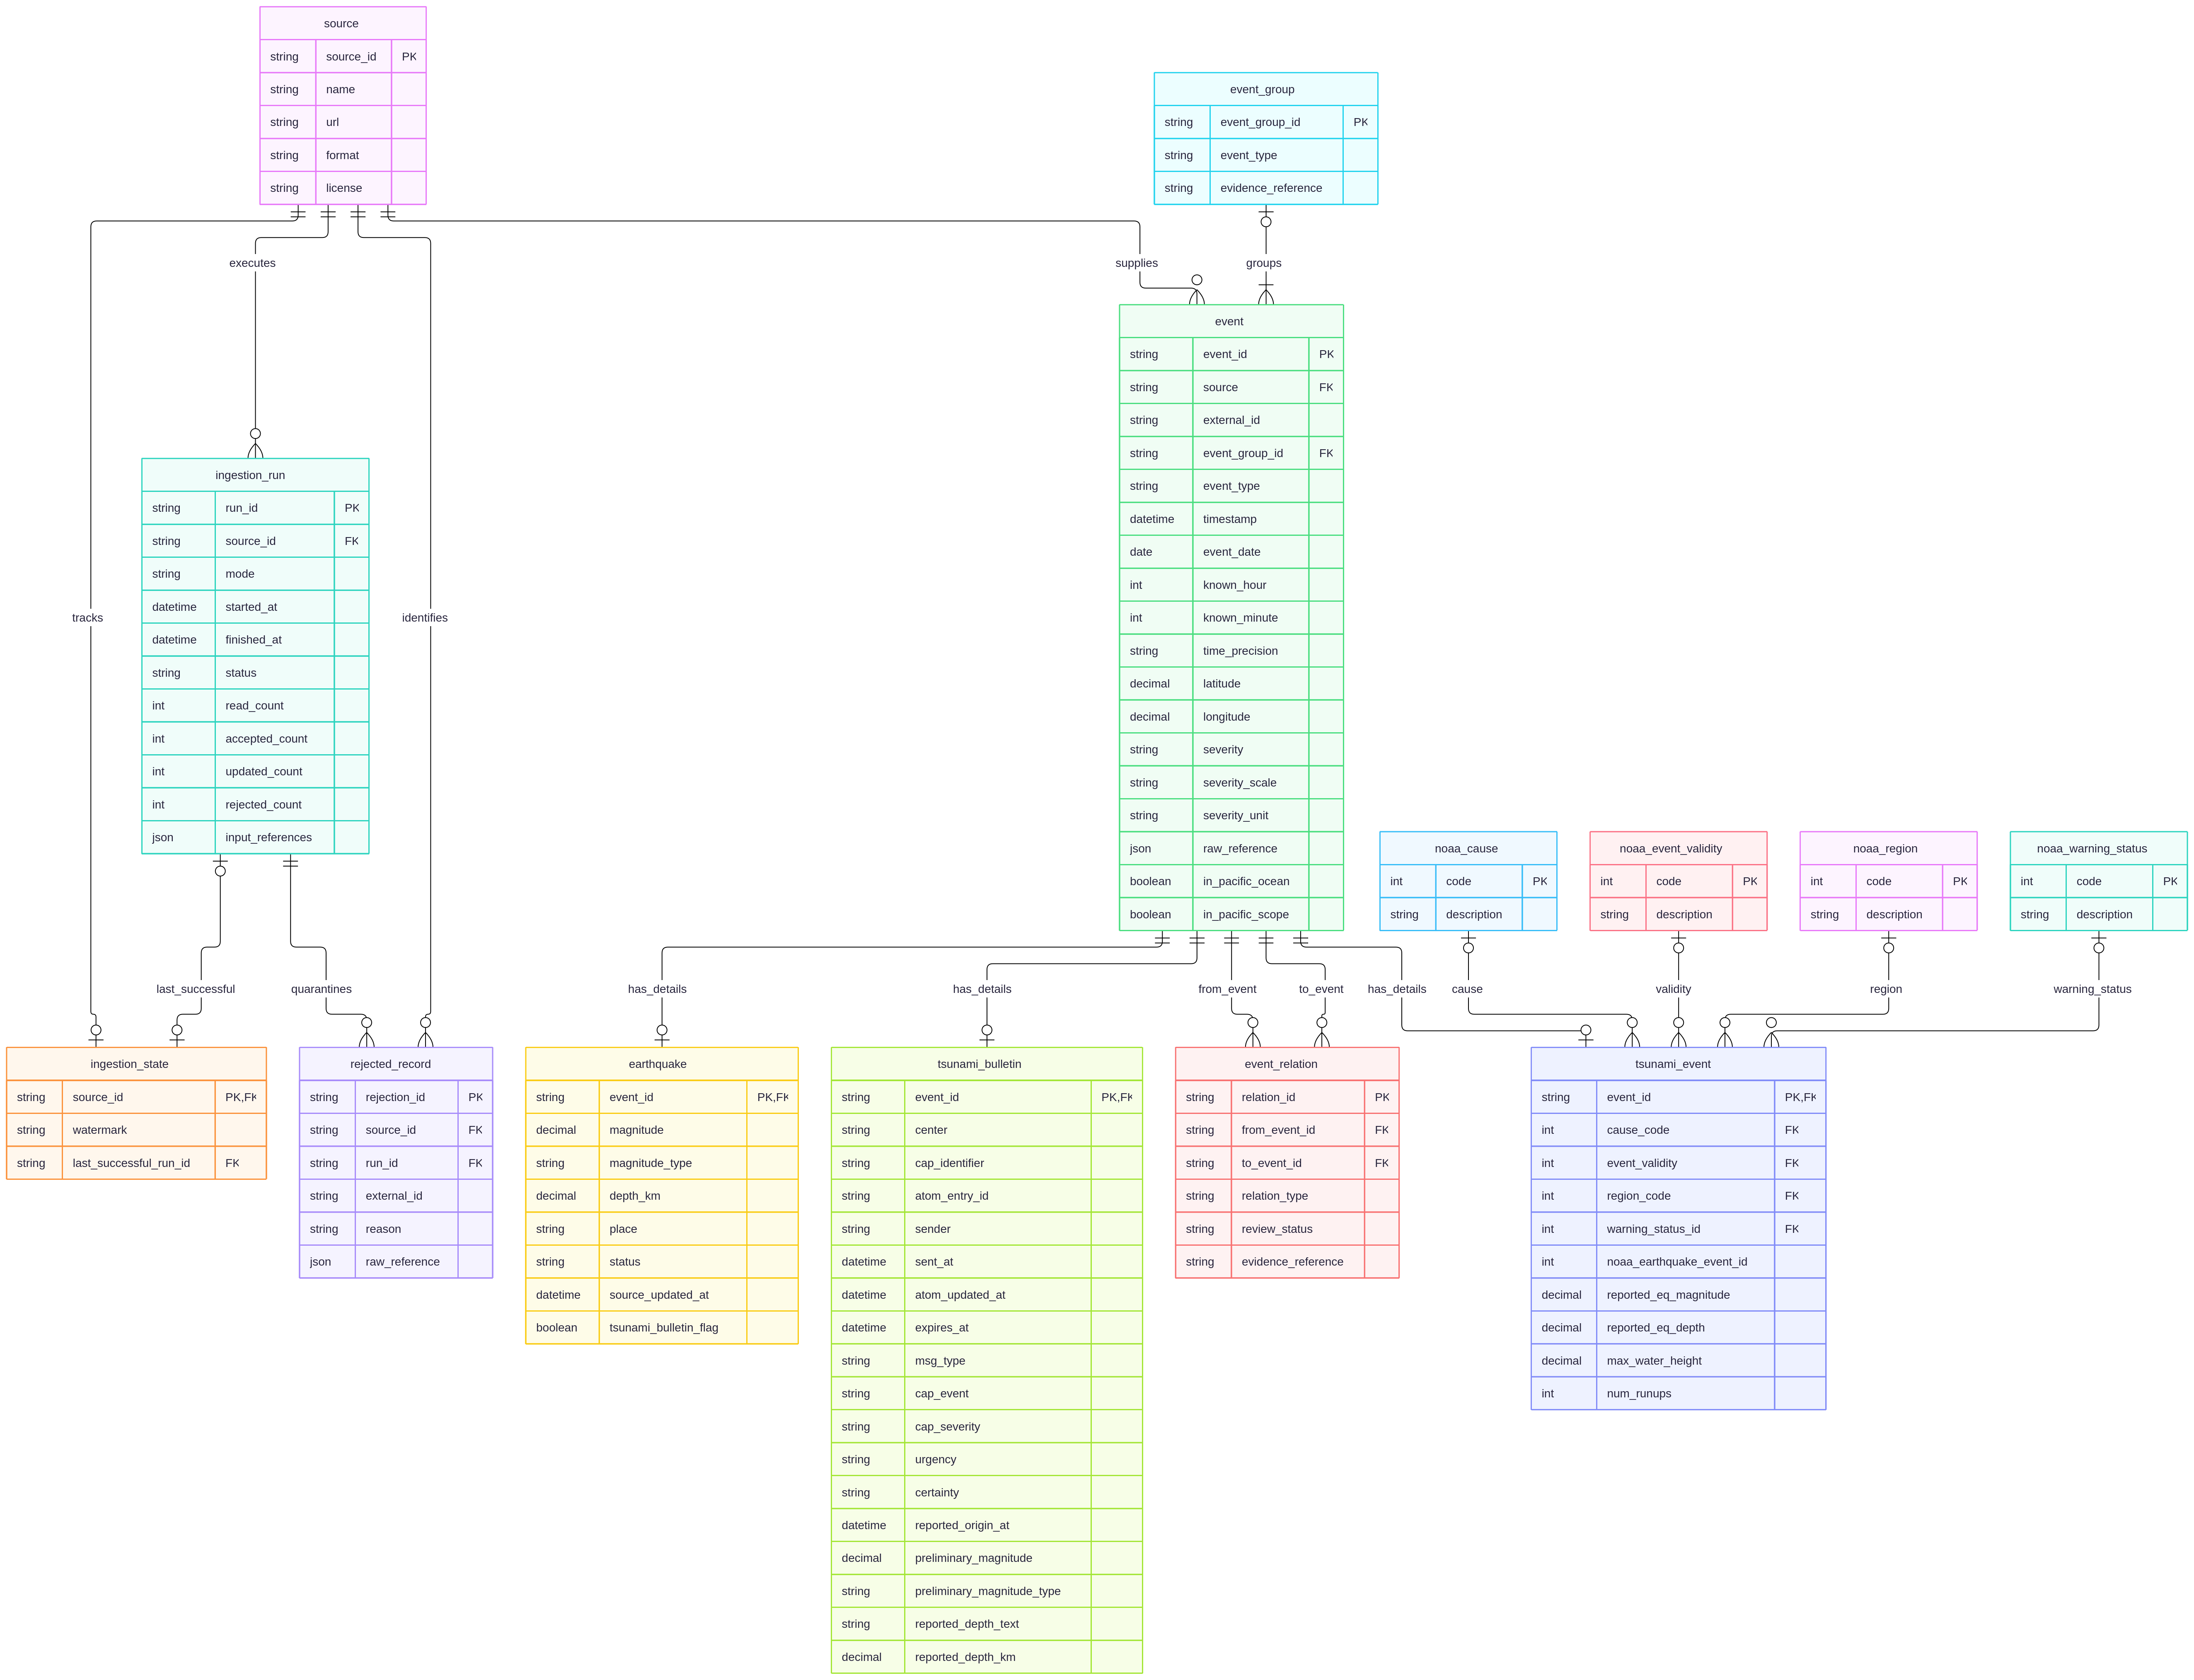
\includegraphics[width=\textheight,height=0.95\textwidth,keepaspectratio]{figures/er_diagram.png}
\caption{Draft entity--relationship diagram (source: \texttt{docs/er\_diagram.md}).}
\label{fig:er}
\end{sidewaysfigure}

\section{Ingestion Contract Draft}
\label{sec:contract}

This section turns the findings of Sections~\ref{sec:historical} and~\ref{sec:incremental} into a per-source contract for \texttt{python ingest.py -{}-mode historical} and \texttt{-{}-mode incremental}.
The rules are proposals for Workshops~2 and~3; they have not been implemented yet.
The duplicate keys follow the canonical model of Section~\ref{sec:mapping}: \texttt{UNIQUE(source, external\_id)}, where \texttt{source} is one of the five controlled source identifiers.

\begin{table}[H]
\centering
\footnotesize
\begin{tabularx}{\textwidth}{@{}>{\raggedright\arraybackslash}p{1.6cm}>{\raggedright\arraybackslash}X>{\raggedright\arraybackslash}X>{\raggedright\arraybackslash}p{2.5cm}>{\raggedright\arraybackslash}p{2.4cm}@{}}
\toprule
Source & Historical strategy & Incremental strategy & Duplicate key & Overlap window \\
\midrule
NOAA HazEL & Query 2010--2025, regions 80--89; iterate \texttt{page} = 1 to \texttt{totalPages} (200 records per page); check that the record count equals \texttt{totalItems} and that no \texttt{id} repeats. & Not an incremental source: records have no update timestamp, so a historical re-run downloads the in-scope records again and compares them by content hash. & (\texttt{noaa\_hazel}, \texttt{id}) & Not needed: every refresh reads the full period. \\
USGS FDSN & One calendar year per request, 2010--2025 (16 requests), $M \geq 6$ in the broad Pacific rectangle; compare each year with the \texttt{count} method; then apply the maritime-scope filter. & Reconciliation query with \texttt{updatedafter}, to catch revisions made after an event has left the real-time feed; watermark: largest stored \texttt{updated}. & (\texttt{usgs\_fdsn}, \texttt{id}) & Query from the watermark minus an overlap (one day proposed), so that late or delayed revisions are not missed. \\
USGS real-time feed & -- & Poll the 4.5+ past-month feed at most once per minute; process an event only when its \texttt{id} is new or its \texttt{updated} is greater than the stored value; compare \texttt{properties} and \texttt{geometry}. & (\texttt{usgs\_realtime}, \texttt{id}) & The whole 30-day file is read on every poll, so recent revisions are always seen again. \\
tsunami.gov (NTWC, PTWC) & -- & Poll each Atom feed every 5 minutes; a CAP \texttt{identifier} not yet stored is a new bulletin, whose CAP message is then downloaded; watermark: latest CAP \texttt{sent} per center. & (\texttt{ntwc} or \texttt{ptwc}, CAP \texttt{identifier}) & All entries present in the feed are re-checked on every poll; bulletins published and removed between two polls cannot be recovered. \\
\bottomrule
\end{tabularx}
\caption{Ingestion contract per source.}
\label{tab:contract}
\end{table}

The Workshop 1 stub saves downloaded responses unchanged in the raw landing zone (\path{data/raw/}) with the name \path{source_YYYYMMDD_HHMMSS.ext}. Under the proposed full ingestion contract, validation failures (for example, invalid coordinates or an unparseable time) would go to \texttt{rejected\_record} with the run identifier and reason without stopping the rest of the batch.
The proposed incremental modes would be idempotent: rerunning them would store no duplicate rows because writes would use upserts on the duplicate key and skip records with unchanged content hashes.

\subsection{Correctness After a Failed Run}
Under the proposed contract, each execution would create an \texttt{ingestion\_run} row (mode, start time, status) before writing data, then close it with its final status and counts.
For every source, one batch and the new watermark in \texttt{ingestion\_state} would be written in the same database transaction, so the watermark would advance only after a successful commit.
The proposed behavior after a failure is:
\begin{itemize}[nosep]
  \item \textbf{Failure before the commit} (network error, timeout or invalid response): the transaction is rolled back, the watermark keeps its previous value, the run is marked as failed, and the next run repeats the same interval.
  \item \textbf{Partially loaded historical load:} batches are committed one partition at a time (one HazEL page, one USGS year), so a failed partition is retried alone while the committed ones are kept; because writes are upserts, repeating a partition creates no duplicates.
  \item \textbf{Failure after downloading:} the raw file is already in the landing zone, so the batch can be reprocessed from it without downloading again.
  \item \textbf{Retries:} each request is retried three times with increasing waits, the team policy of Section~\ref{sec:historical}, before the run is marked as failed.
\end{itemize}
The proposed database-backed \texttt{-{}-mode status} command would report each source's watermark, last successful run and row counts. The Workshop 1 stub currently lists saved raw files only.

\section{Indicator Proposal}
\label{sec:indicator}
The \textbf{Tsunami Relevance Level} (TRL) summarizes how much attention a recent earthquake deserves from a tsunami-monitoring perspective.
It is a monitoring aid, \textbf{not a tsunami prediction or warning}; official warnings come only from the tsunami warning centers.

\textbf{Inputs.} For each earthquake with $M \geq 6$ inside the Pacific scope: magnitude (moment magnitude preferred), focal depth, historical tsunami association, and the official bulletin linked to it, if any.

\textbf{Rule (all thresholds are parameters in the configuration).}
\begin{itemize}[nosep]
  \item Magnitude points: 1 for $6.0 \leq M < 7.0$, 2 for $7.0 \leq M < 8.0$, 3 for $M \geq 8.0$.
  \item Depth point: 1 if the depth is at most 70~km, since shallow earthquakes are more likely to displace the seafloor.
  \item History point: 1 if at least one probable or definite (validity 3--4) earthquake-caused HazEL tsunami lies within 300~km.
  \item Level: \textbf{LOW} for 0--2 points, \textbf{MODERATE} for 3, \textbf{HIGH} for 4--5. An earthquake deeper than 300~km is at most LOW.
  \item Official override: a linked CAP bulletin with \texttt{severity} of \texttt{Moderate}, \texttt{Severe} or \texttt{Extreme} (the categories above \texttt{Minor}) is shown as \textbf{OFFICIAL ALERT} and is never displayed below HIGH. The product classification (information, advisory, watch or warning) is displayed separately; it is not inferred from CAP \texttt{severity}.
\end{itemize}

\textbf{Examples from the samples.} The 2011 Tohoku earthquake ($M$ 9.1, 29~km deep) scores 5 points and is HIGH. Its history point can be supported without using its own tsunami (HazEL 5413): the saved HazEL records 5412 and 5931 are definite, earthquake-caused tsunamis of 9 March 2011 within 300~km of its epicenter.
The 25 October 2026 Bonin Islands earthquake ($M$ 6.5, 492~km deep) would score 2 points (it has two 2023 Izu Islands tsunamis within 300~km), but its depth limits it to LOW, consistent with the PTWC information statement (\texttt{Minor} / \texttt{Unlikely}).

\textbf{Validation against historical events.} The indicator will be applied to the 1,930 USGS $M \geq 6$ earthquakes of 2010--2025 (Table~\ref{tab:usgs-counts}). NOAA--USGS candidate links require review before verified identities can be used as ground truth; each earthquake's own tsunami is excluded from its history point.
Two measures will be reported: the share of tsunami-associated earthquakes rated MODERATE or HIGH, and the share of earthquakes without a tsunami rated HIGH.
A sensitivity analysis will vary the magnitude limits by $\pm 0.5$, the depth limit between 50 and 100~km, and the history radius between 200 and 500~km.

\textbf{Limitations.} The level uses proxies only: it ignores the focal mechanism, the distance to the coast and local bathymetry; preliminary magnitudes and depths change after publication; the 2010--2025 history is short and uneven across regions; landslide and volcanic tsunamis are not rated; and the official override depends on U.S. warning centers whose coverage does not include every Pacific coast.

\section{Architecture Overview}
Figure~\ref{fig:architecture} adapts the course reference architecture to the four sources; it is exported from the Mermaid source in \path{docs/architecture.md}.
In the proposed architecture, all components run locally with Docker Compose: a scheduler (proposed: an Apache Airflow DAG) calls \texttt{ingest.py -{}-mode incremental}, and the Plotly Dash dashboard reads only from the database. Workshop 1 implements the raw-download stub, not the integrated stack.

\begin{figure}[H]
\centering
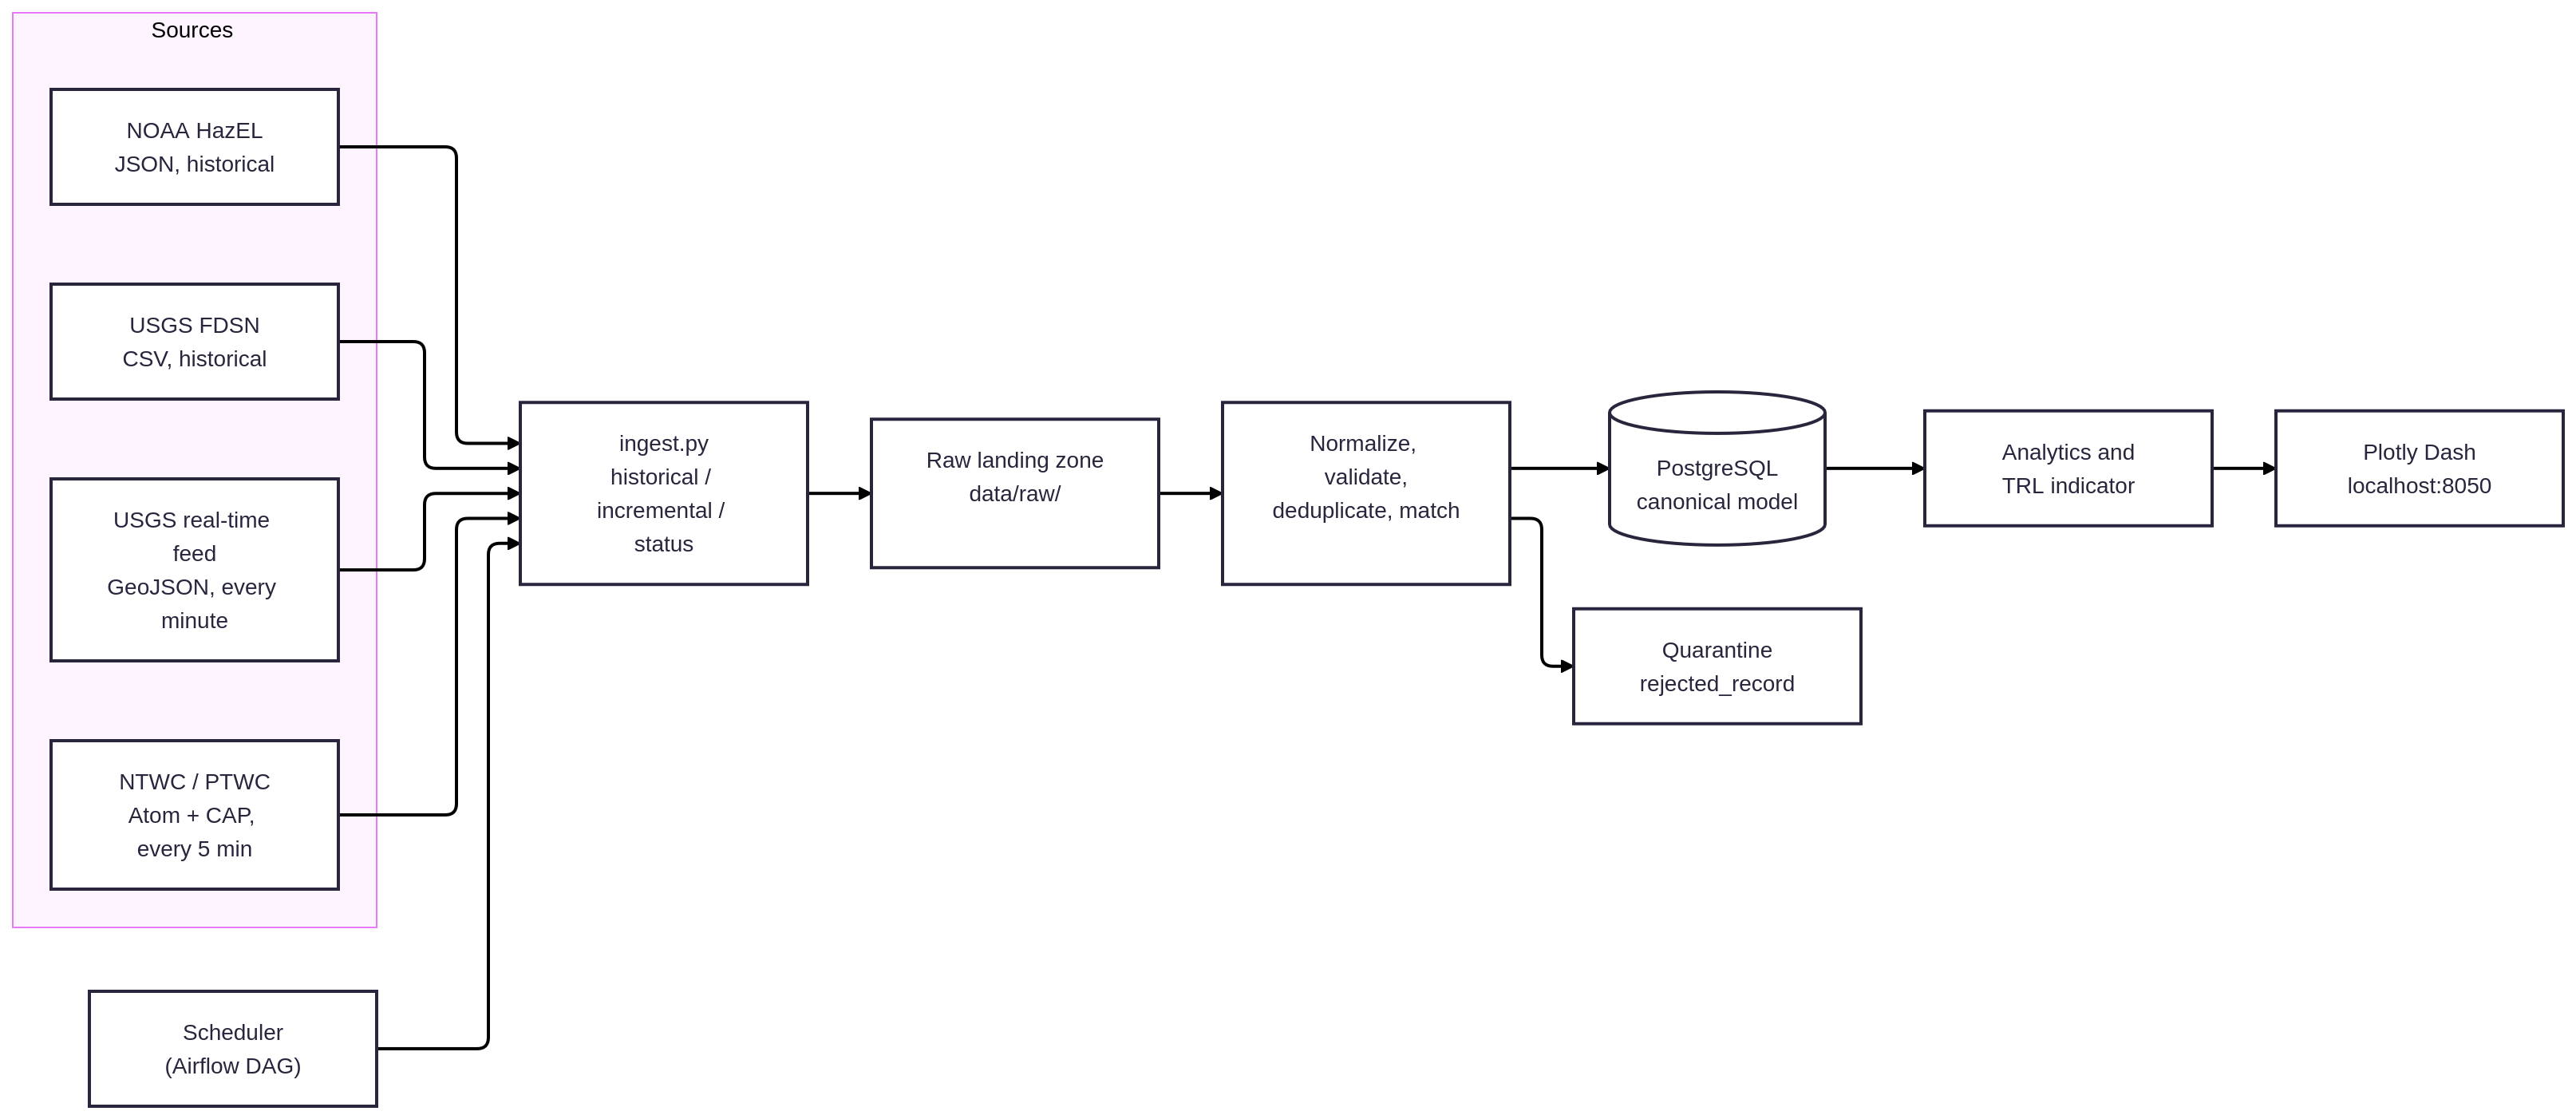
\includegraphics[width=\textwidth]{figures/architecture.png}
\caption{High-level architecture (source: \texttt{docs/architecture.md}).}
\label{fig:architecture}
\end{figure}

\chapter{Results}
\label{ch:results}

\section{Empirical Update Behavior}
\label{sec:empirical-updates}
Four snapshots were saved on 7 November 2026 at 05:04 and 14:03 UTC,
12 November at 03:38 UTC, and 16 November at 01:37 UTC.
They provide three consecutive comparison intervals. The two 7 November
captures are about nine hours apart (00:04 and 09:03 in Bogot\'a, UTC$-5$).
Table~\ref{tab:first-increment} reports only this first interval.

\begin{table}[H]
\centering
\begin{tabular}{lrr}
\toprule
 & USGS feed & NTWC/PTWC feeds \\
\midrule
First snapshot (records) & 714 & 1 per center \\
Second snapshot (records) & 726 & 1 per center \\
New identifiers & 22 & 0 per center \\
Modified USGS features & 25 & -- \\
Absent identifiers & 10 & 0 per center \\
\bottomrule
\end{tabular}
\caption{Observed changes between the two 7 November snapshots.}
\label{tab:first-increment}
\end{table}

A new USGS event has an \texttt{id} absent from the preceding snapshot.
A modified event keeps its \texttt{id} but changes \texttt{properties}
or \texttt{geometry}; the 25 modified events in the first interval
include changes to magnitude, depth, or location.
An absent event was present in the earlier file but not in the later one.
The feed lists $M \geq 4.5$ events of the past 30 days, so an event can leave it by aging out, by a magnitude revision below 4.5, or by deletion.
Across the three intervals, 288 events became absent: 282 had origin times older than the 30-day cutoff of the later snapshot, making their absence consistent with aging out of the feed. These 282 were not checked individually in the catalog, so their continued presence cannot be confirmed from the saved evidence. The other six were looked up in the USGS FDSN catalog.
None of those six had been deleted; all were still \texttt{reviewed} events whose magnitude had been revised from 4.5--4.6 to 4.4 (\texttt{mb}), below the feed threshold (for example, \texttt{us6000u4kh} near Vanuatu).
An absence alone does not establish whether an event aged out, fell below the magnitude threshold or was deleted.
The saved catalog responses are in \path{workshop_1/samples/usgs_fdsn_absent_events_20261116.json}.
The notebook applies the Pacific scope to the latest snapshot rather than to each interval: 492 of the 679 events of 16 November are inside the scope (Section~\ref{sec:hazard}).
The comparisons and examples are in Section 5 of
\path{notebooks/01_source_profiling.ipynb}.

Both NTWC and PTWC retained the same CAP identifier between the two
7 November captures. Different CAP identifiers appeared in the
12 and 16 November captures. These are newly observed bulletins;
without evidence linking them to the same incident, they must not be
called revisions of one event. Feed entries may also appear and
disappear between saved captures.

\section{Source Profiling and Data Quality}
\label{sec:profiling}

\subsection{Profiling Summary}
The saved samples were examined in \path{notebooks/01_source_profiling.ipynb} (Sections 3--7): missing values, field types and ranges, duplicated identifiers, timestamp formats and time zones, coordinate validity and units. Per-field null percentages are available in the three historical/USGS HTML profiles; the six distinct CAP messages are summarized below.
Table~\ref{tab:profile} summarizes the result.
No source has duplicated identifiers inside a snapshot, and no coordinate is outside the WGS84 ranges or at $(0, 0)$; the only invalid locations are 9 HazEL events without coordinates.
USGS and tsunami.gov timestamps are represented in UTC, but in different formats: the FDSN CSV uses ISO~8601 with \texttt{Z}, the real-time feed uses epoch milliseconds, and tsunami.gov uses ISO~8601 (with \texttt{Z} in the Atom feed and the offset \texttt{-00:00} in CAP). HazEL splits dates and times into six columns (\texttt{year} to \texttt{second}, with fractional seconds and sometimes missing clock components) without an explicit time-zone field; the notebook interprets complete times as UTC for comparison, an assumption that still needs source confirmation.
Depth is given in kilometers by USGS, as an integer without unit by HazEL, and as text with its unit (\texttt{473 kilometers}) by the CAP messages.
Magnitude comes with its type in USGS (6 types in each sample: \texttt{mww}, \texttt{mwc}, \texttt{mb}, \texttt{mwb}, \texttt{mw}, \texttt{ms} in the catalog; \texttt{mb} for 562 of 679 feed events), without type in HazEL, and as a preliminary value with its type (\texttt{Ml}, \texttt{Mwp}) in tsunami.gov.

\begin{table}[H]
\centering
\small
\begin{tabularx}{\textwidth}{@{}lrr>{\raggedright\arraybackslash}X@{}}
\toprule
Source & Records & Dupl.\ ids & Notes \\
\midrule
NOAA HazEL & 221 & 0 & 57 profiled columns (50 source fields and 7 derived fields); 2010-01-02 to 2025-12-12. Impact fields (deaths, damage, houses) are 63--99.5\% null; \texttt{warningStatusId} 76.5\% null; \texttt{eqMagnitude} and \texttt{eqDepth} 15.8\% null (tsunamis without an earthquake cause); 9 events without coordinates. \\
USGS FDSN & 343 & 0 & 24 columns; 2010--2011, $M$ 6.0--9.1, depth 2.8--644.6~km. \texttt{magError} 100\% null; \texttt{dmin} and \texttt{horizontalError} 99.4\% null; \texttt{depthError} 80.8\% null. All events \texttt{reviewed}. \\
USGS real-time & 679 & 0 & 32 columns; origin times 17 October to 15 November 2026, $M$ 4.5--7.0, depth 1--642~km. \texttt{tz} 100\% null; \texttt{alert} 90.1\% null; \texttt{mmi} 88.5\% null; \texttt{felt}, \texttt{cdi} 84.8\% null. All events \texttt{reviewed}; 5 with \texttt{tsunami} = 1. \\
tsunami.gov & 6 & 0 & Six distinct CAP messages (three per center) in the four snapshots; each feed holds only its latest messages, so the 200-record minimum cannot apply. All six are information statements (\texttt{Tsunami Information}, \texttt{Minor} / \texttt{Unlikely}). \\
\bottomrule
\end{tabularx}
\caption{Profiling summary of the four samples (16 November snapshot for the USGS real-time feed; distinct messages of the four snapshots for tsunami.gov).}
\label{tab:profile}
\end{table}

The six distinct saved CAP messages contain 37 parsed CAP fields. Thirty-two fields have a value in all six messages (0\% missing). Among the remaining fields, \texttt{headline} is empty in three messages (50\%); \texttt{WEAK53} and \texttt{NWSUGC} are absent as XML elements in three each (50\%); \texttt{WECA42} is absent in four (66.7\%); and \texttt{ProductDefinition} is absent in three and present with an empty \texttt{value} element in three (100\% without a value). These percentages use six distinct CAP identifiers, not the eight repeated snapshot observations. An absent element and an empty element are distinguished here; neither is an explicit XML null value. The notebook does not store a complete per-field CAP null-percentage table.

\subsection{Data-Quality Problems}
Eight problems were identified in the saved samples. The notebook's Section 6 profiles the main quality issues; its Section 7 examines the CAP--USGS date mismatch as a candidate cross-source link. The CAP expiration inconsistency was checked directly against the saved NTWC message.

\begin{table}[H]
\centering
\small
\begin{tabularx}{\textwidth}{@{}c>{\raggedright\arraybackslash}p{2.1cm}>{\raggedright\arraybackslash}X>{\raggedright\arraybackslash}X@{}}
\toprule
\# & Source & Problem & Example record \\
\midrule
1 & NOAA HazEL & Official warning status missing: 169 of 221 events (76\%) have no \texttt{warningStatusId}. & Event 4522 (Solomon Islands, 3 January 2010): definite tsunami (validity 4) with no warning status. \\
2 & NOAA HazEL & Erroneous or doubtful events: 9 events with \texttt{eventValidity} $\leq 2$ (8 questionable, 1 erroneous entry). & Event 5407 (South Island, New Zealand, 21 February 2011): questionable tsunami (validity 2). \\
3 & NOAA HazEL & Time of day or coordinates missing: 23 events have only a date, and 9 events have no coordinates. & Event 4762 (Lake 513, Hualcan glacier, Peru, 13 April 2010): no hour or minute. Event 5739 (Cheju Strait, 2 January 2010): no latitude or longitude. \\
4 & USGS FDSN & Columns that are always or almost always empty: \texttt{magError} is 100\% null, \texttt{dmin} and \texttt{horizontalError} 99.4\%. & Event \texttt{official2011\allowbreak 0311054624120\_30} (Tohoku, 11 March 2011): empty \texttt{magError}, \texttt{horizontalError} and \texttt{dmin}. \\
5 & tsunami.gov & Location as free text and depth as text with its unit; the location text uses miles. & NTWC message \texttt{PAAQ-1-to0j1g}: ``75 miles SW of Eureka, California''; CAP \texttt{EventDepth} = ``13 kilometers''. \\
6 & tsunami.gov & Suspected CAP origin-date error: the stated time is about one day earlier than a plausible USGS earthquake candidate. & PTWC message \texttt{PHEB-1-26297050}, sent 25 October 2026 at 02:27 UTC, gives \texttt{EventOriginTime} 24 October 02:09 UTC; USGS candidate \texttt{us6000u4r9} occurred on 25 October at 02:09:24 UTC. \\
7 & USGS real-time & The \texttt{tsunami} flag can be misread: it means that a bulletin may exist, not that a tsunami happened (5 of 679 events in the 16 November snapshot). & Event \texttt{us6000u4r9} (Bonin Islands, $M$ 6.5, depth 492~km): \texttt{tsunami} = 1, while the PTWC message for it says \texttt{Minor} / \texttt{Unlikely}. \\
8 & tsunami.gov &
Invalid CAP validity interval: an observed bulletin has an
expiration time earlier than its publication time. &
NTWC snapshot: \texttt{sent} =
2026-11-13 23:30:02 UTC and \texttt{expires} =
2026-11-13 12:30:02 UTC, an 11-hour inconsistency. \\
\bottomrule
\end{tabularx}
\caption{Data-quality problems found in the samples.}
\label{tab:quality}
\end{table}

In addition, 36 of the 221 HazEL events have a non-earthquake cause (Section~\ref{sec:hazard}), so their magnitude and depth are empty by nature and must not be treated as missing values.
\paragraph{Additional interpretation notes.}

The NOAA historical catalog contains events generated by
earthquakes, landslides, volcanoes, and other mechanisms.
Missing earthquake magnitude or depth is therefore not
automatically a data-quality error.

NOAA event 6045 refers to the 2025 Tracy Arm landslide tsunami
in Alaska. Its reported 481 m maximum run-up represents an
extreme local elevation reached by the water, not the height
of a wave propagating across the Pacific \cite{tracy}.

NOAA event 5413, corresponding to the 2011 Tohoku tsunami,
has \texttt{numRunups} = 6429. This field counts run-up records;
it is not a water-height measurement.

For CAP messages, the validation rule requires the expiration
timestamp to be greater than or equal to the publication
timestamp. Inconsistent messages should be flagged without
silently changing the original source data.

\subsection{Cross-Source Overlap}
\label{sec:overlap}
The exploratory matching in Section 7 of the notebook uses time precision, epicenter distance of at most 100~km, and magnitude agreement for records without exact times. It produces 28 candidate NOAA--USGS FDSN pairs from 2010--2011; two NOAA records have more than one eligible USGS event and require manual review. The median exact-time difference is 0.075~s, the median distance is 0~km, and the median magnitude difference is 0. HazEL depth is within 2~km of USGS depth in 25 of the 28 selected pairs.

The CAP--USGS examples below come from the saved 7 November snapshot. The NTWC bulletin has a close USGS candidate; the PTWC bulletin needs a wider diagnostic search because its stated CAP origin date is about one day earlier than the likely USGS earthquake. This remains a candidate link, not a confirmed identity. Table~\ref{tab:pairs} lists six illustrative candidates ($\Delta t$ is record B time minus record A time).

\begin{table}[H]
\centering
\small
\begin{tabularx}{\textwidth}{@{}c>{\raggedright\arraybackslash}p{4.1cm}rr>{\raggedright\arraybackslash}p{1.9cm}>{\raggedright\arraybackslash}X@{}}
\toprule
\# & Record A / Record B & $\Delta t$ & Distance & Magnitude A / B & What differs \\
\midrule
1 & tsunami.gov \texttt{PAAQ-1-to0j1g} / USGS feed \texttt{nc75462637} & $-1.3$~s & 8.7~km & 4.5 Ml / 4.96 mw & Magnitude value and type, depth (13 vs 10~km), location text \\
2 & HazEL 5413 / USGS \texttt{official2011\allowbreak 0311054624120\_30} & $+0.02$~s & 0.0~km & 9.1 / 9.1 mww & Identifier format; HazEL time rounded to 0.1~s and magnitude without type \\
3 & HazEL 4682 / USGS \texttt{official2010\allowbreak 0227063411530\_30} & $+0.03$~s & 0.0~km & 8.8 / 8.8 mww & Depth 22 vs 22.9~km (HazEL integer) \\
4 & HazEL 5406 / USGS \texttt{usp000huc2} & $+0.21$~s & 15.9~km & 6.8 / 6.9 mww & Epicenter, depth (28 vs 26~km) and magnitude \\
5 & HazEL 5931 / USGS \texttt{usp000hvkh} & $+0.68$~s & 0.0~km & 6.3 / 6.5 mwc & Magnitude (0.2 lower in HazEL); HazEL time without decimals \\
6 & tsunami.gov \texttt{PHEB-1-26297050} / USGS feed \texttt{us6000u4r9} & $+1$~day $+24$~s & 35.8~km & 7.0 Mwp / 6.5 mww & Origin date (problem 6), preliminary magnitude 0.5 higher, depth (473 vs 492~km) \\
\bottomrule
\end{tabularx}
\caption{Candidate cross-source links from the historical sample and 7 November snapshot; identity is not yet confirmed.}
\label{tab:pairs}
\end{table}

These candidates show why magnitude should be compared with tolerance rather than required to match exactly. An anomalous CAP time also calls for checking location and magnitude before proposing a link. Final matching and ambiguous pairs belong in the Canonical Mapping.

\chapter{Discussion}
\label{ch:discussion}

\section{Revised or Missing Records and Proposed Ingestion Strategy}
The observed USGS revisions show why origin time or new identifiers
alone would miss updates. The following rules are proposed for the
ingestion contract; they have not yet been implemented or verified.

\paragraph{USGS real-time feed.}
The proposed ingestion strategy will compare all event identifiers in
each downloaded feed and use \texttt{updated} rather than origin
\texttt{time} as a revision watermark. It should compare both
\texttt{properties} and \texttt{geometry}, and use idempotent writes
keyed by a source identifier and event ID. A content hash of selected
normalized fields could distinguish substantive changes from metadata
updates. An event absent from a later feed should be retained while
its status is investigated: an absence can mean aging out of the 30-day window,
a magnitude revision below 4.5, or a deletion. An FDSN lookup by event ID
distinguishes these cases; it was done manually for the six early absences of
Section~\ref{sec:empirical-updates} and will be automated during ingestion.

\paragraph{USGS FDSN catalog.}
A proposed overlapping query with \texttt{updatedafter} could detect
revisions after an event leaves the real-time feed; its schedule,
overlap duration, and completeness still need validation. The two USGS
endpoints may describe the same earthquake. A per-source key
\texttt{(source, id)} prevents repeats within each source but does not
merge those observations automatically. The Canonical Mapping must
specify how USGS identifiers are normalized and how cross-source
duplicates are recognized, without assuming a final table structure here.

\paragraph{tsunami.gov.}
The proposed comparison will track CAP identifiers and publication
times per center across all entries in each Atom feed. A new CAP
identifier is a new bulletin observation; a possible revision of the
same event requires separate evidence, such as a shared incident
identifier. Conditional requests using \texttt{Last-Modified} may
reduce repeated downloads, but HTTP 304 behavior has not been tested.
Polling cannot recover a bulletin published and removed between polls.

\paragraph{NOAA HazEL and failed runs.}
HazEL has no update timestamp, so a proposed historical refresh would
compare records by identifier and content. The ingestion design should
advance a source watermark only with a successful data commit and use
idempotent writes so a failed batch can be retried. These failure and
deduplication rules are specified as proposals in Section~\ref{sec:contract}.

\section{Risks and Mitigation}
\begin{table}[H]
\centering
\small
\begin{tabularx}{\textwidth}{@{}>{\raggedright\arraybackslash}p{2.6cm}>{\raggedright\arraybackslash}X>{\raggedright\arraybackslash}X@{}}
\toprule
Risk & Impact & Mitigation \\
\midrule
Source outage & Missing updates; the dashboard shows stale data without noticing. & Retries with increasing waits; failed runs keep the previous watermark; the data-health panel shows the watermark age (Section~\ref{sec:contract}). \\
Rate limits & Blocked or truncated requests (USGS FDSN returns at most 20,000 events per query). & One USGS request per year with a \texttt{count} check; polling at most once per minute (USGS) and every 5 minutes (tsunami.gov); identified User-Agent; caching of raw files. \\
Schema change & Parsing failures or silently wrong fields (the two centers already use different CAP parameters, and Marine Regions stores ``Easter'' instead of ``Eastern''). & Validation before loading, \texttt{rejected\_record} with the reason, raw files kept for reprocessing, and tests with recorded fixtures. \\
License and attribution & Use outside the terms of a source (Marine Regions asks users not to redistribute its files). & Licenses recorded per source; boundaries downloaded by a script instead of committed; credit lines in the report and README. \\
Ambiguous identifiers & Wrong links between records (two NOAA records have more than one USGS candidate; a PTWC CAP origin date is one day off). & Links stored as \texttt{identity\_candidate} with a review status; no automatic merging; groups only after review. \\
Record revisions & Outdated values (25 modified events in nine hours, including 21 relocations; six magnitudes lowered below 4.5). & Watermark on \texttt{updated}, content hash, re-reading the 30-day feed and an FDSN lookup for early absences (Section~\ref{sec:empirical-updates}). \\
Data volume & Memory exhaustion: the 100~km test on the approximately 145~MB local maritime GeoJSON exhausted a 7~GB laptop when run together with other programs. & Prepared geometries, simplified boundaries for display, and heavy notebook steps run alone. \\
\bottomrule
\end{tabularx}
\caption{Risks and mitigation.}
\label{tab:risks}
\end{table}

\chapter{Conclusions and Open Questions}
\label{ch:conclusions}
\section{Main Decisions}
\begin{itemize}[nosep]
  \item \textbf{Scope:} the Pacific is defined by three official Marine Regions maritime regions plus a 100~km monitoring margin, which keeps 205 of the 221 NOAA events and 319 of the 343 USGS historical events (Section~\ref{sec:hazard}).
  \item \textbf{Sources:} NOAA HazEL and USGS FDSN as historical sources; the USGS 4.5+ past-month feed and the NTWC/PTWC Atom and CAP feeds as incremental sources (Chapter~\ref{ch:sources}).
  \item \textbf{Units:} HazEL depth is in kilometers and maximum water height in meters, as documented by the HazEL search forms (Section~\ref{sec:severity}).
  \item \textbf{Data model:} one \texttt{event} row per source observation, three domain tables, and reviewed links through \texttt{event\_group} and \texttt{event\_relation} instead of automatic merging (Section~\ref{sec:mapping}).
  \item \textbf{Incremental design:} watermark on the USGS \texttt{updated} field, upserts on \texttt{(source, external\_id)}, content hashes, and the watermark advancing only after a successful commit (Section~\ref{sec:contract}).
  \item \textbf{Indicator:} the Tsunami Relevance Level, based on magnitude, depth, historical tsunami association and official bulletins (Section~\ref{sec:indicator}).
\end{itemize}

\section{Key Findings}
Records change after publication: across the three intervals 22 to 121 new and 25 to 123 modified USGS events appeared, and the revisions of the first interval arrived between 1 and 29 days after the earthquake. Of 288 absences, 282 are consistent with aging out of the 30-day window but were not individually checked in the catalog; the other six were confirmed there as magnitude downgrades below 4.5, not deletions.
The tsunami.gov feeds change rarely but contain inconsistencies that must be flagged and preserved, not corrected.
Cross-source matching works well for NOAA and USGS (28 candidate pairs with median time and distance differences close to zero), but two NOAA records have more than one USGS candidate, so links require review.

\section{Open Questions for Workshop 2}
\begin{itemize}[nosep]
  \item Build the Docker Compose stack and the PostgreSQL schema from the ER diagram (Figure~\ref{fig:er}).
  \item Implement \texttt{--mode historical} beyond the raw landing zone: parsing, validation, quarantine and idempotent loading, with \texttt{config/sources.yaml} and \texttt{.env.example} completed.
  \item Fix the final cross-source matching rule and decide how ambiguous candidates are reviewed.
  \item Automate the FDSN lookup that explains events absent from the feed.
  \item Validate and calibrate the indicator thresholds against the 2010--2025 record.
  \item Reduce the memory cost of the 100~km scope test so that the pipeline runs comfortably on the team's laptops.
\end{itemize}

\chapter{Reflection}
\label{ch:reflection}
\textbf{What worked.} Querying every source for real before designing anything was the most valuable decision of the workshop: the samples revealed problems that the documentation does not mention, such as the one-day error in a PTWC origin time, magnitudes revised weeks after an earthquake, and the HazEL units, which are stated only in the search forms and not in the API description.
Keeping every response unchanged in \path{workshop_1/samples/} allowed us to recheck earlier claims whenever a new snapshot arrived, and several statements of the report were corrected this way.

\textbf{What was difficult.} The sources disagree on almost everything that looks simple: time formats, time zones, magnitude types, identifiers and coordinate conventions.
The geographic scope took several iterations, from a hand-drawn polygon to the official Marine Regions boundaries, and the antimeridian and the size of the boundary file (which exhausted a 7~GB laptop) required care.
Coordinating three people on one report and one notebook also produced conflicts, such as a duplicate PDF uploaded through the web interface and simultaneous builds of the report.

\textbf{Lessons learned.} Every number in the report should be traceable to a notebook output or a saved file; assumptions must be stated as proposals until they are verified; absence of data is not evidence of deletion; and small, frequent commits with clear messages make teamwork much easier than large uploads.


    % -------------------------------------------------------------------
    % References
    % -------------------------------------------------------------------
\begin{thebibliography}{9}
\bibitem{hazel} National Geophysical Data Center / World Data Service. \emph{NCEI/WDS Global Historical Tsunami Database}. NOAA National Centers for Environmental Information. doi:10.7289/V5PN93H7. Accessed through the HazEL API, \url{https://www.ngdc.noaa.gov/hazel/view/swagger}, 8 November 2026.
\bibitem{usgsfdsn} U.S.\ Geological Survey. \emph{API Documentation -- Earthquake Catalog}. \url{https://earthquake.usgs.gov/fdsnws/event/1/}. Accessed 8 November 2026.
\bibitem{usgscredit} U.S.\ Geological Survey. \emph{Acknowledging or Crediting USGS}. \url{https://www.usgs.gov/information-policies-and-instructions/acknowledging-or-crediting-usgs}. Accessed 8 November 2026.
\bibitem{usgsfeed} U.S.\ Geological Survey. \emph{Real-time Notifications, Feeds, and Web Services (GeoJSON summary feed)}. \url{https://earthquake.usgs.gov/earthquakes/feed/v1.0/geojson.php}. Accessed 7 and 9 November 2026.
\bibitem{hazelforms} NOAA National Centers for Environmental Information. \emph{HazEL tsunami event search} and \emph{earthquake search} forms. \url{https://www.ngdc.noaa.gov/hazel/view/hazards/tsunami/event-search} and \url{https://www.ngdc.noaa.gov/hazel/view/hazards/earthquake/search}. Accessed 16 November 2026.
\bibitem{tsunamigov} NOAA National Weather Service, Tsunami Warning Centers. \emph{Tsunami event feeds}. \url{https://www.tsunami.gov/}. Accessed 7 and 9 November 2026.
\bibitem{marineregions}
Flanders Marine Institute (2021).
\emph{Global Oceans and Seas, version 1}.
Marine Regions.
\url{https://doi.org/10.14284/542}.
Licensed under CC BY 4.0.
Accessed 16 November 2026.

\bibitem{taupo}
Smithsonian Institution, Global Volcanism Program (2022).
\emph{Report on Taupo (New Zealand),
30 November--6 December 2022}.
\url{https://volcano.si.edu/showreport.cfm?gvpvar=GVP.WVAR20221130-241070}.

\bibitem{tracy}
Shugar, D. H., et al.\ (2026).
\emph{A 481 m-high landslide-tsunami in a
cruise ship--frequented Alaska fjord}.
\textit{Science}. doi:10.1126/science.aec3187.
\url{https://doi.org/10.1126/science.aec3187}.
Accessed 16 November 2026.
\end{thebibliography}

    % -------------------------------------------------------------------
    % Appendices
    % -------------------------------------------------------------------
    \begin{appendices}
\chapter{Real Response Snippets}
\label{app:snippets}
Short excerpts of the unmodified responses stored in \path{workshop_1/samples/}.
Each excerpt shows one record; ``\ldots'' marks fields or lines left out for brevity.

\section{NOAA HazEL -- tsunami events}
File \path{noaa_tsunamis_pacific_2010_2025.json}, record of the 2011 Tohoku tsunami, and the pagination fields of the response:
\begin{lstlisting}
{"items": [ ...
  {"id": 5413, "year": 2011, "month": 3, "day": 11, "hour": 5, "minute": 46,
   "latitude": 38.297, "longitude": 142.373, "causeCode": 1,
   "eventValidity": 4, "eqMagnitude": 9.1, "eqDepth": 29,
   "maxWaterHeight": 39.26, "warningStatusId": null, "regionCode": 85,
   "numRunups": 6429, "country": "JAPAN", "locationName": "HONSHU ISLAND", ...},
  ... ],
 "page": 1, "totalPages": 2, "itemsPerPage": 200, "totalItems": 221}
\end{lstlisting}

\section{USGS FDSN -- earthquake catalog}
File \path{usgs_earthquakes_2010_2011_m6_pacific.csv}, header and a highly compatible earthquake candidate:
\begin{lstlisting}
time,latitude,longitude,depth,mag,magType,nst,gap,dmin,rms,net,id,updated,place,type,horizontalError,depthError,magError,magNst,status,locationSource,magSource
2011-03-11T05:46:24.120Z,38.297,142.373,29,9.1,mww,541,9.5,,1.16,official,official20110311054624120_30,2026-10-16T10:38:09.160Z,"2011 Great Tohoku Earthquake, Japan",earthquake,,,,,reviewed,us,official
\end{lstlisting}
The two records are a highly compatible candidate match: they have the same origin minute, epicenter and magnitude, and HazEL \texttt{eqDepth} (29) equals the USGS depth in km. The notebook retains this link as a candidate requiring review because other USGS events also satisfy its exploratory time-and-distance rule; identity has not been formally verified.

\section{USGS real-time feed}
The file \path{usgs_realtime_20261107_050434.geojson} contains feed
metadata and its first feature. Times are in epoch milliseconds;
coordinates are longitude, latitude, and depth in km.
\begin{lstlisting}
{"type": "FeatureCollection",
 "metadata": {"generated": 1794027872000,
   "url": "https://earthquake.usgs.gov/earthquakes/feed/v1.0/summary/4.5_month.geojson",
   "title": "USGS Magnitude 4.5+ Earthquakes, Past Month", "status": 200, "count": 714, ...},
 "features": [
  {"type": "Feature", "id": "us7000twmr",
   "properties": {"mag": 4.8, "place": "36 km WNW of Poso, Indonesia",
     "time": 1793992021269, "updated": 1794002237040, "tsunami": 0,
     "magType": "mb", "status": "reviewed", "type": "earthquake", ...},
   "geometry": {"type": "Point", "coordinates": [120.4589, -1.2393, 10]}},
  ... ]}
\end{lstlisting}

\section{tsunami.gov -- PTWC Atom feed}
File \path{ptwc_20261107_050434.xml}, the single entry of the feed (an information statement); the linked CAP message is stored in \path{ptwc_cap1_20261107_050434.xml}:
\begin{lstlisting}
<entry>
  <title>BONIN ISLANDS  JAPAN REGION</title><updated>2026-10-25T02:27:01Z</updated>
  <geo:lat>28.</geo:lat>
  <geo:long>139.9</geo:long>
  <summary type="xhtml"> ... <strong>Category:</strong> Information<br/>
    <strong>Bulletin Issue Time: </strong> 2026.10.25 02:27:01 UTC <br/>
    <strong>Preliminary Magnitude: </strong>7.0(Mwp)<br/> ... </summary>
  <id>urn:uuid:ba64bc82-07f7-45fb-ab6c-25420fca6851</id>
  <link rel="related" title="CapXML document" type="application/cap+xml"
        href="https://www.tsunami.gov/events/PHEB/2026/10/24/26297050/1/WEGM42/PHEBCAP.xml" />
</entry>
\end{lstlisting}

\chapter{Reproducing the Workshop 1 Results}
\label{app:reproduce}
From the repository root, with Python 3.12 to 3.14:
\begin{lstlisting}
python3 -m venv .venv
source .venv/bin/activate
pip install -r requirements.txt

# Use the existing raw samples in workshop_1/samples/ for the reported figures.
# Marine Regions boundaries for the geographic scope (about 145 MB)
python3 workshop_1/download_marine_regions.py

\end{lstlisting}
The profiling notebook \path{notebooks/01_source_profiling.ipynb} is run from the \path{notebooks/} directory with the \texttt{.venv} kernel.
To collect new samples for later analysis, run \texttt{download\_historical\_samples.py}, \texttt{download\_incremental\_samples.py}, or the Workshop 1 \texttt{ingest.py} raw-download stub separately. New snapshots can change which files the notebook discovers; \texttt{-{}-force} may overwrite existing historical samples and is not a reproduction step for the figures above. The current \texttt{ingest.py -{}-mode status} lists raw files only.
    \end{appendices}

\end{document}
